\documentclass[article, a4paper]{llncs}

\usepackage{ucs} 
\usepackage[utf8x]{inputenc} % Включаем поддержку UTF8  
\usepackage[russian]{babel}  % Включаем пакет для поддержки русского языка  
\usepackage{csquotes}
\usepackage{graphicx}
\graphicspath{/} 
%--Настройка полей--%
\usepackage[left=35mm, top=30mm, right=35mm, bottom=30mm, nohead, footskip=7mm]{geometry}
%--для нечетных страниц left - слева, для четных - справа--%
\setcounter{tocdepth}{3}
\setlength{\parindent}{0pt} % Убираем отстубы для красных строк
\pagestyle{plain} %включаем нумерацию страниц
\setlength{\parskip}{5pt plus 2pt minus 1pt}
\newcommand{\Csh}{C{\lserif\#}}
\newcommand{\keywords}[1]{\par\addvspace\baselineskip
\noindent\keywordname\enspace\ignorespaces#1}

\title{
		\usefont{OT1}{bch}{b}{n}
		\normalfont \normalsize \textsc{ITMO University} \\ [25pt]
		\huge Fibonacci heap \\
}
\author{
		\normalfont 								
		\normalsize
        Grigory Panov\\[-5pt]		
        \normalsize
}
\institute{
\today
}

\date{}

\begin{document}
\maketitle
    \section{Постановка задачи}
    В данной курсовой работе необходимо было:
    \begin{itemize}
        \item Реализовать Фибоначчиеву кучу;
            \begin{itemize}
                \item написать программу на языке \Csh{};
                \item протестировать ее на корректность;
                \item протестировать время работы.
            \end{itemize}
        \item Подготовить отчет, содержащий исходный код и краткую информацию с подробностями реализации и результатами тестов.
    \end{itemize}
    
    \section{Краткая сводка}
    Фибоначчиева куча — набор из подвешенных деревьев удовлетворяющих свойству: каждый предок не больше своих детей. Это означает, что минимум всей кучи это один из корней этих деревьев. Одним из главных преимуществ Фибоначчиевой кучи — гибкость её структуры из-за того, что на деревья не наложены никакие ограничения по форме. Например, Фибоначчиева куча может состоять только из деревьев в каждом из которых по одному элементу. Такая гибкость позволяет выполнять некоторые операции лениво, оставляя работу более поздним операциям. В структуре постоянно хранится ссылка на минимальный элемент, что позволяет обеспечить операцию взятия минимума за O(1). 
    \section{Подробности реализации} 
    Структура была реализована на языке \Csh{} на основании таких ресурсов, как https://neerc.ifmo.ru/  // http://wikipedia.org/ // https://www.cs.usfca.edu/~galles/visualization/FibonacciHeap.html . Структура данных состоит из 3х классов - FibHeap, FibNode и MyLinkedList. Также класс MyLinkedList использует в своей реализации класс Node.
    FibNode - класс представляющий из себя ноду дерева. FibHeap - класс, представляющий из себя фибоначеву кучу. Поддерживает слеудющие доступные операции: Push, GetMin, GetMinNode, Merge, Pop, DecreaseKey. Для хранения верхнего списка, а также списка детей фибоначевой ноды используется самописный MyLinkedList. Изначально в реализации использовался LinkedList из стандартной коллекции, однако, как оказалось, в нем не поддерживается операция слияния двух списков за 0(1) необходимая для операции Push. Первый элемент верхнего списка является всегда минимальным. Все операции, кроме операции Push(Delete), выполняются за константное время.
    \section{Подробности тестирования}
    В качестве тестов корректности работы структуры данных было произведено покрытие реализованной функциональности юнит-тестами, которые отвечают за корректность производимых операций. В ходе тестирования я старался сконцентрироваться на том, какие операции мог бы производить пользователь с данной системой и какой результат он бы ожидал от нее. К примеру, проверка операций добавления одного или нескольких элементов, проверка операции получения минимума при разных условиях - с соседями и без них, с детьми и без них, удаление элементов из верхнего уровня и нет и тд. Для вспомогательных классов, FibNode, это тестирование поведения, которое ожидается от них использующими их классами. 
    \section{Подробности тестирования времени работы}
    Для тестирования времени работы были взяты основные операции структуры и замеры производились с помощью класса System.Diagnostics.Stopwatch в тиках, которые являлись 0,0001 миллисекунды. 
    Алгоритм тестирования представлен ниже:
    1) Выполнение заданного количества операций (от 10000 до 335000), причем с вероятностью 95 процентов эта операция - Push и с вероятностью 5 процентов - Pop.
    2) Выполнение замера скорости выполнения 10000 операций Push/Pop с вероятностью каждой в 50 процентов. 
    3) Повторения пункта 2) для получения средней скорости выполнения данной операции после 10ти кратного измерения.
    4) Повторение 1-3 с большим количеством операций. Шаг = 5000.
    
    Как итог - мы получаем похожую на логарифмическую зависимость скорости выполнения, в среднем, 5000 операций Push и 5000 операций Pop.
    \begin{figure}[h]
        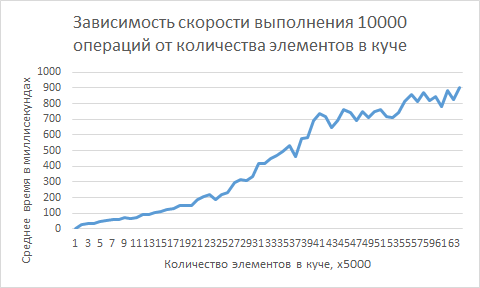
\includegraphics[width=14cm, height=8cm]{1.png}
        \centering
    \end{figure}

   Итого получаем структуру:\\
    Операция: Амортизированная сложность \\
    makeHeap: O(1) \\
    insert: O(1) \\
    getMin: O(1) \\
    merge: O(1) \\
    extractMin: $O( \log n )$ \\
    decreaseKey: O(1) \\
    delete: $O( \log n )$ \\

   
\end{document}
	